% =============================================================================
% 81-lampiran-pemenuhan.tex — Tabel Pemenuhan + Bukti Implementasi
% =============================================================================

% ─────────────────────────────────────────────────────────────────────────────
\section*{Lampiran A: Tabel Pemenuhan Kebutuhan/Permintaan Dosen Pemilik Proyek}
\label{lamp:tabel-pemenuhan}
\setcounter{table}{0}
\renewcommand{\thetable}{A.\arabic{table}}

{\footnotesize
\renewcommand{\arraystretch}{1.3}
\begin{longtable}{|p{0.6cm}|p{4.0cm}|p{1.8cm}|p{5.8cm}|}
  \caption{Pemenuhan Kebutuhan/Permintaan Dosen Pemilik Proyek} \\
  \hline
  \textbf{No.} & \textbf{Kebutuhan/Permintaan Dosen Pemilik Proyek} & \textbf{Status} & \textbf{Keterangan} \\
  \hline
  \endfirsthead
  \hline
  \textbf{No.} & \textbf{Kebutuhan/Permintaan Dosen Pemilik Proyek} & \textbf{Status} & \textbf{Keterangan} \\
  \hline
  \endhead
  \hline
  \endfoot

  \multicolumn{4}{|l|}{\textbf{TERCAPAI}} \\
  \hline

  1 & Penambahan 2 asesmen (GPIUS-2 \& SRS) & Tercapai & Kedua instrumen ditambahkan ke katalog dengan butir soal, opsi jawaban, dan rentang interpretasi sesuai spesifikasi ahli domain, melengkapi PSS-10 dan SRQ-29. \\
  \hline
  2 & Visualisasi hasil \textit{real-time} & Tercapai & Hasil ditampilkan instan setelah penyelesaian melalui visualisasi grafik (\textit{gauge}, \textit{radar}, diagram batang) menggunakan Recharts. \\
  \hline
  3 & Permohonan laporan lengkap via surel & Tercapai & Pengguna mengajukan permintaan laporan melalui formulir tervalidasi; permintaan tersimpan pada tabel \texttt{report\_requests} untuk diproses administrator. \\
  \hline
  4 & Dasbor antrean permintaan (verifikasi/setuju/tolak) & Tercapai & Administrator dapat melihat, menyetujui, atau menolak permintaan; persetujuan memicu generasi PDF dan pengiriman surel. \\
  \hline
  5 & Visualisasi grafik admin + \textit{filtering} & Tercapai & Dasbor menyajikan visualisasi agregat dengan filter berdasarkan instrumen, wilayah, usia, kategori, rentang skor, dan rentang tanggal. \\
  \hline
  6 & \textit{Dropdown} domisili bertingkat & Tercapai & Formulir demografis menyediakan pemilihan domisili dua level (provinsi $\rightarrow$ kota/kabupaten) berbasis dataset 38 provinsi (klasifikasi BPS). \\
  \hline
  7 & Opsi Lainnya' (manual) & Tercapai & Input provinsi dan kota/kabupaten menyediakan opsi `Lainnya (ketik manual)'' dengan nilai sentinel \texttt{\_\_other\_\_} untuk pengisian wilayah yang tidak terdaftar. \\
  \hline
  8 & \textit{Save as Image} pada grafik & Tercapai & Komponen grafik dilengkapi tombol unduh gambar (komponen \texttt{SaveChartButton}, pustaka \texttt{html-to-image}, resolusi 2$\times$). \\
  \hline
  9 & \textit{Dynamic Sorting} (asc/desc) & Tercapai & Tabel hasil mendukung pengurutan dinamis pada enam kolom secara \textit{ascending} dan \textit{descending} (sisi-server via \texttt{sortBy}/\texttt{sortDir}, didukung sisi-klien). \\
  \hline
  10 & Modul Manajemen Asesmen (CRUD) & Tercapai & Administrator melakukan operasi CRUD penuh atas tes, butir soal, opsi jawaban, dan rentang interpretasi. \\
  \hline
  11 & Ekspor .CSV dan .XLS & Tercapai & Sistem menyediakan ekspor data dalam format CSV dan XLSX menggunakan pustaka SheetJS. \\
  \hline
  12 & \textit{Filtered Download} (dinamis) & Tercapai & Data yang diunduh mengikuti filter aktif melalui kondisi filter yang sama dengan tampilan tabel (\texttt{buildFilterConditions}). \\
  \hline
  13 & Penyimpanan data sementara (\textit{resume}) & Tercapai & Jawaban tersimpan otomatis pada setiap perubahan via prosedur \texttt{saveProgress}, memungkinkan pengguna melanjutkan sesi yang terputus. \\
  \hline
  14 & Modul log aktivitas (\textit{audit}) & Tercapai & Setiap modifikasi direkam dalam tabel \texttt{audit\_logs} mencakup aktor, aksi, entitas, serta nilai sebelum dan sesudah. \\
  \hline
  15 & Pelaporan komprehensif per pengguna & Tercapai & Setiap pengguna memiliki laporan komprehensif mencakup visualisasi data pribadi, analisis per-dimensi, dan interpretasi mendetail. \\
  \hline
  16 & Ekspor PDF/XLSX/CSV Individual & Tercapai & Hasil mendalam dapat diunduh dalam format PDF (via \texttt{@react-pdf/renderer}), XLSX, dan CSV. \\
  \hline
  17 & RBAC bertingkat & Tercapai & RBAC empat peran (\texttt{super\_admin}, \texttt{admin}, \texttt{psychiatrist}, \texttt{researcher}) dengan lima tingkat \textit{middleware}. \textit{Super Admin} berakses penuh; Admin tidak dapat mengelola akun dan hanya melihat aktivitas sendiri; \textit{Researcher}/Psikiater tidak dapat membuat/mengedit asesmen maupun mengelola akun, hanya melihat aktivitas sendiri. \\
  \hline
  18 & Modul Manajemen Akun (\textit{Super Admin}) & Tercapai & \textit{Super Admin} dapat membuat, memperbarui, dan mengatur hak akses akun administrator melalui modul \textit{Account Management}. \\
  \hline

  \multicolumn{4}{|l|}{\textbf{BELUM TERCAPAI}} \\
  \hline

  19 & Peringatan otomatis pada pertanyaan belum terisi & Belum Tercapai & Umpan balik eksplisit per-butir belum tercapai karena kompleksitas sinkronisasi status pengisian antara penyimpanan sisi-klien (\texttt{localStorage}) dan persistensi sisi-server secara simultan. Sebagai mitigasi, tombol `Kirim Asesmen'' dinonaktifkan secara \textit{default} dan hanya aktif setelah seluruh pertanyaan terjawab, sehingga pengiriman tidak lengkap tetap tercegah. \\
  \hline
  20 & \textit{Import} Data .XLS/.XLSX & Belum Tercapai & Fitur impor data massal belum tercapai karena kompleksitas validasi skema terhadap data historis yang beragam format dan struktur, yang berpotensi menimbulkan inkonsistensi apabila tidak divalidasi secara ketat. Fitur ditangguhkan ke iterasi berikutnya demi menjaga integritas data penelitian. \\
  \hline
  21 & \textit{Contact Us} & Belum Tercapai & Fitur korespondensi surel dua arah belum tercapai karena memerlukan integrasi layanan surel dua arah yang melampaui cakupan waktu kerja praktik. Diidentifikasi sebagai \textit{backlog} prioritas tinggi untuk fase berikutnya. \\
  \hline
  22 & \textit{Direct Mail Responder} & Belum Tercapai & Sama dengan butir 21: memerlukan integrasi surel dua arah yang melampaui cakupan waktu kerja praktik, dan diidentifikasi sebagai \textit{backlog} prioritas tinggi untuk fase berikutnya. \\
  \hline

\end{longtable}
}

\vspace{1cm}
\begin{flushright}
\begin{tabular}{c}
Menyetujui, \\
Dosen Pemilik Proyek \\[2.5cm]
Dr. Yasinta Astin Sokang, S.Psi., M.Psi., Psikolog \\
\end{tabular}
\end{flushright}

\clearpage

% ─────────────────────────────────────────────────────────────────────────────
\section*{Lampiran B: Bukti Implementasi Permintaan Dosen Pemilik Proyek}
\label{lamp:bukti-implementasi}
\setcounter{figure}{0}
\renewcommand{\thefigure}{B.\arabic{figure}}

\begin{figure}[H]
\centering
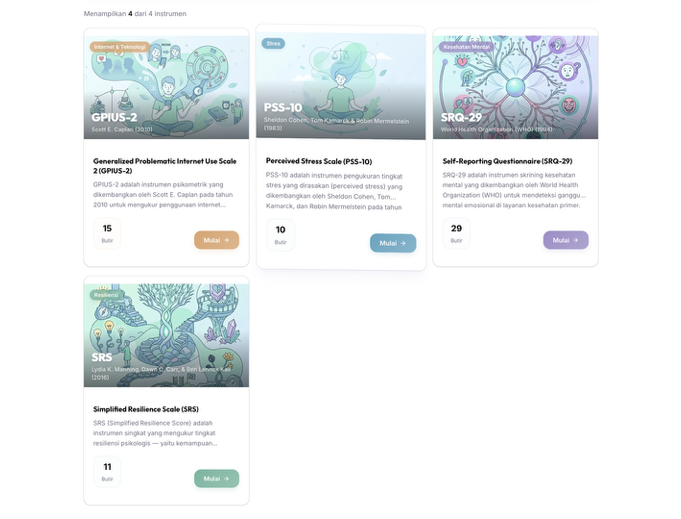
\includegraphics[width=0.9\textwidth]{figures/bukti_01_penambahan_asesmen.png}
\caption{Bukti Butir 1: Penambahan asesmen GPIUS-2 dan SRS}
\label{fig:bukti-01}
\end{figure}

\begin{figure}[H]
\centering
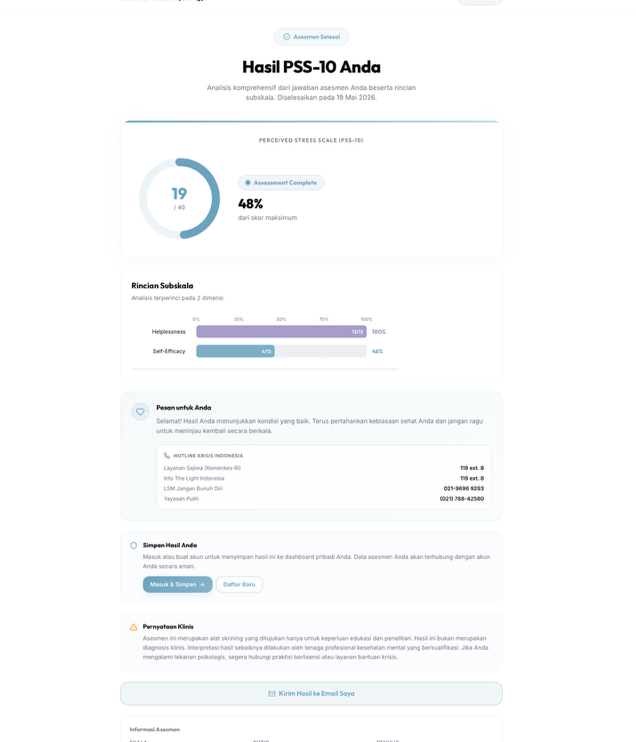
\includegraphics[width=0.9\textwidth]{figures/bukti_02_visualisasi_realtime.png}
\caption{Bukti Butir 2: Visualisasi hasil asesmen real-time}
\label{fig:bukti-02}
\end{figure}

\begin{figure}[H]
\centering
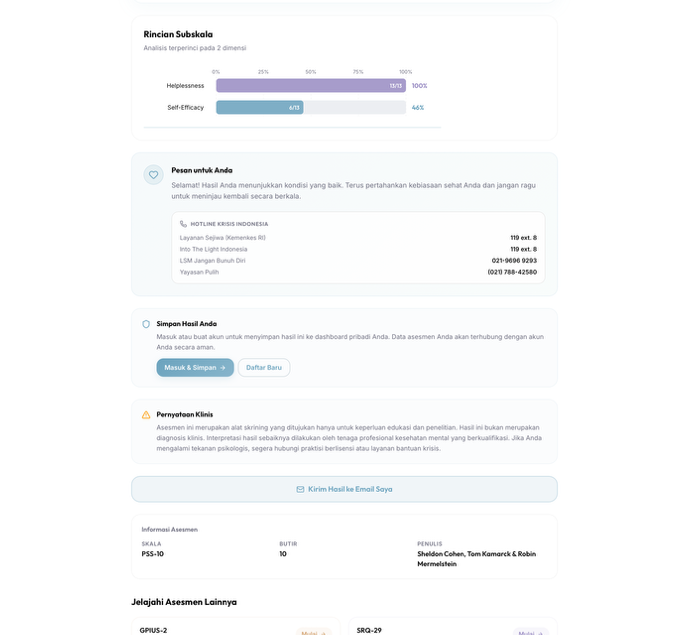
\includegraphics[width=0.9\textwidth]{figures/bukti_03_permohonan_laporan.png}
\caption{Bukti Butir 3: Formulir permohonan laporan}
\label{fig:bukti-03}
\end{figure}

\begin{figure}[H]
\centering
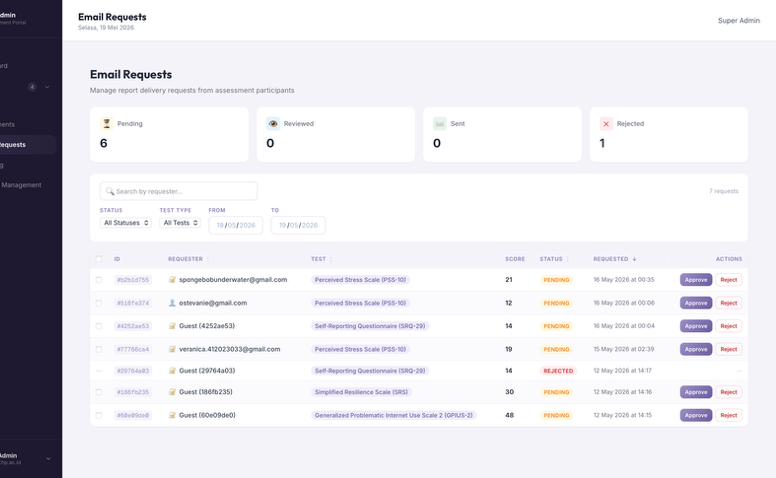
\includegraphics[width=0.9\textwidth]{figures/bukti_04_dasbor_antrean.png}
\caption{Bukti Butir 4: Dasbor manajemen antrean permintaan}
\label{fig:bukti-04}
\end{figure}

\begin{figure}[H]
\centering
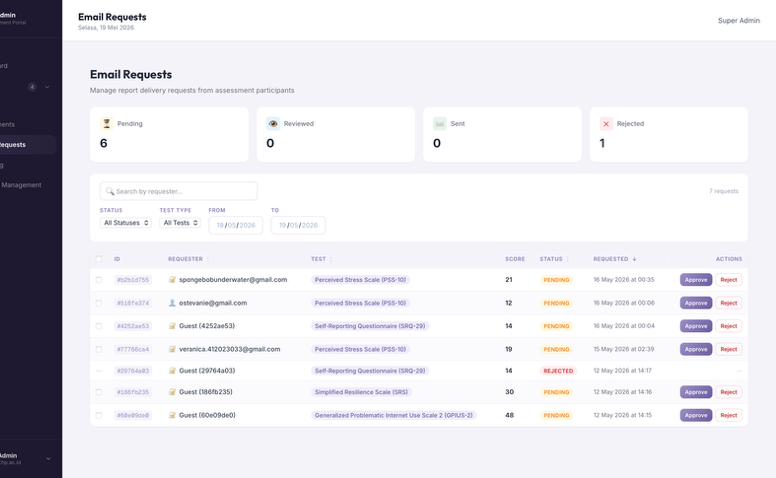
\includegraphics[width=0.9\textwidth]{figures/bukti_05_grafik_admin.png}
\caption{Bukti Butir 5: Visualisasi grafik dengan filtering}
\label{fig:bukti-05}
\end{figure}

\begin{figure}[H]
\centering
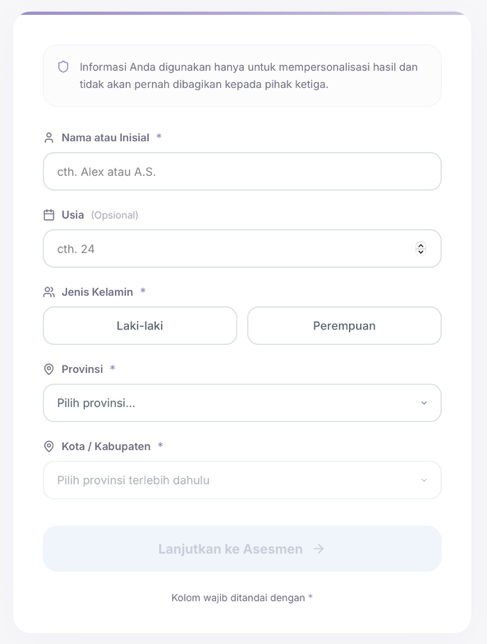
\includegraphics[width=0.9\textwidth]{figures/bukti_06_dropdown_domisili.png}
\caption{Bukti Butir 6: Dropdown domisili bertingkat}
\label{fig:bukti-06}
\end{figure}

\begin{figure}[H]
\centering
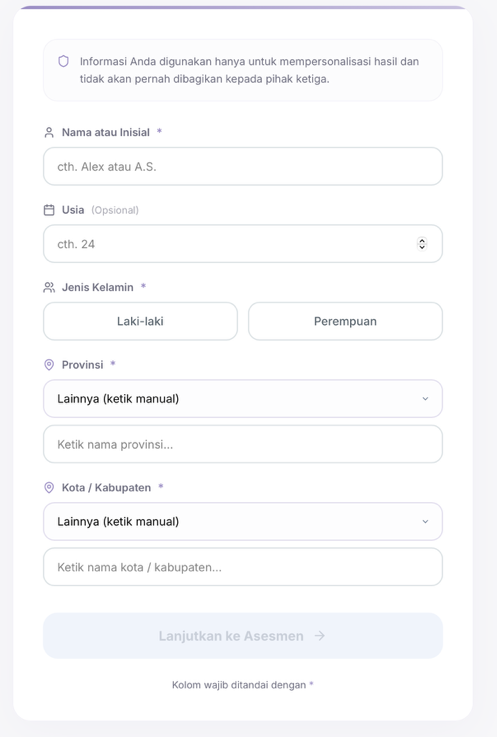
\includegraphics[width=0.9\textwidth]{figures/bukti_07_opsi_lainnya.png}
\caption{Bukti Butir 7: Opsi Lainnya' pengisian manual}
\label{fig:bukti-07}
\end{figure}

\begin{figure}[H]
\centering
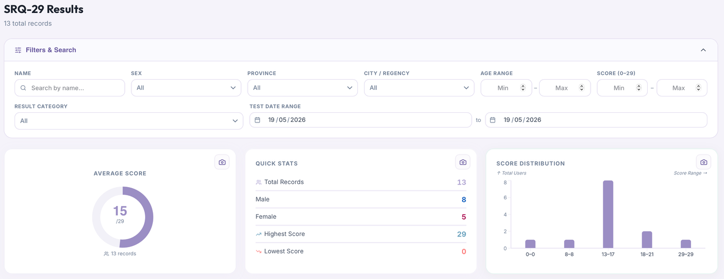
\includegraphics[width=0.9\textwidth]{figures/bukti_08_save_as_image.png}
\caption{Bukti Butir 8: Fitur Save as Image pada grafik}
\label{fig:bukti-08}
\end{figure}

\begin{figure}[H]
\centering
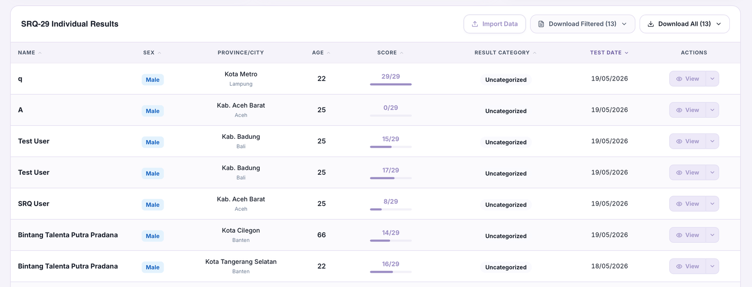
\includegraphics[width=0.9\textwidth]{figures/bukti_09_dynamic_sorting.png}
\caption{Bukti Butir 9: Dynamic Sorting kolom tabel}
\label{fig:bukti-09}
\end{figure}

\begin{figure}[H]
\centering
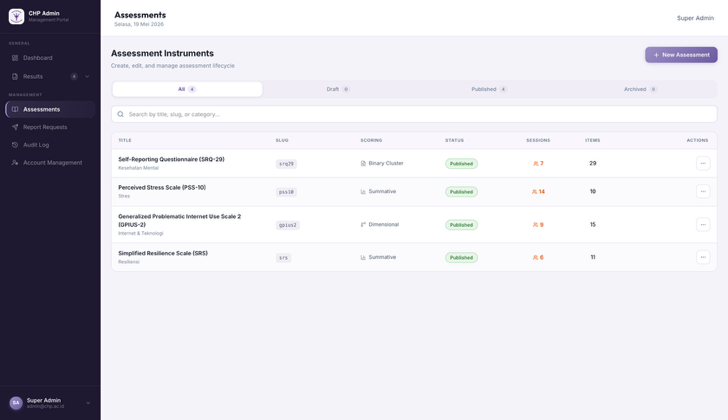
\includegraphics[width=0.9\textwidth]{figures/bukti_10a_manajemen_asesmen.png}
\caption{Bukti Butir 10: Modul Manajemen Asesmen (daftar)}
\label{fig:bukti-10a}
\end{figure}

\begin{figure}[H]
\centering
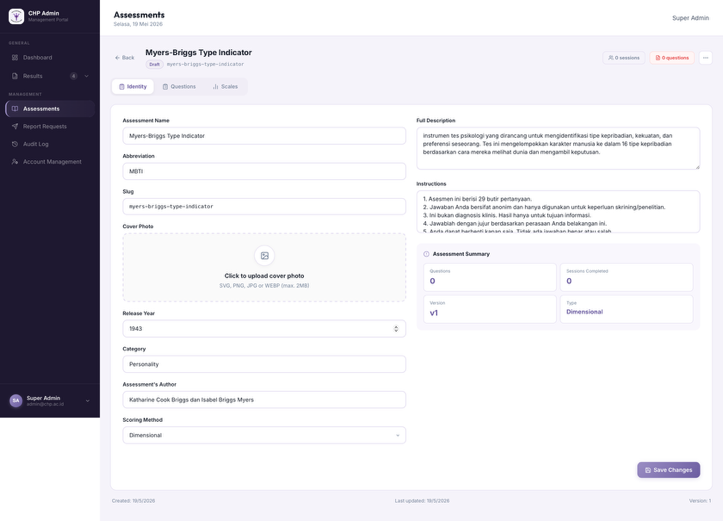
\includegraphics[width=0.9\textwidth]{figures/bukti_10b_manajemen_asesmen.png}
\caption{Bukti Butir 10: Modul Manajemen Asesmen (penyuntingan)}
\label{fig:bukti-10b}
\end{figure}

\begin{figure}[H]
\centering
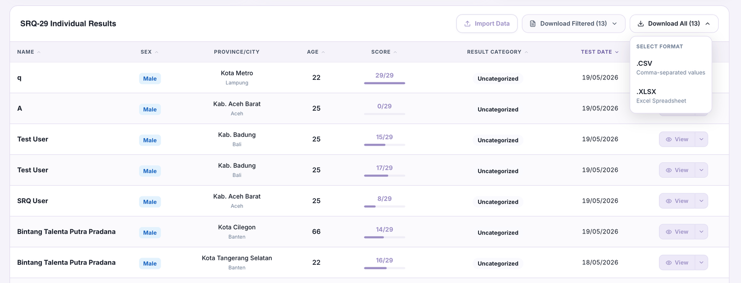
\includegraphics[width=0.9\textwidth]{figures/bukti_11_ekspor_csv_xls.png}
\caption{Bukti Butir 11: Ekspor data CSV dan XLS}
\label{fig:bukti-11}
\end{figure}

\begin{figure}[H]
\centering
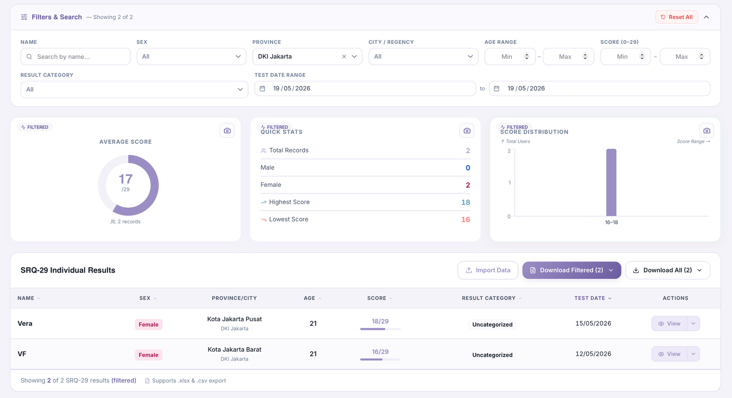
\includegraphics[width=0.9\textwidth]{figures/bukti_12_filtered_download.png}
\caption{Bukti Butir 12: Filtered Download}
\label{fig:bukti-12}
\end{figure}

\begin{figure}[H]
\centering
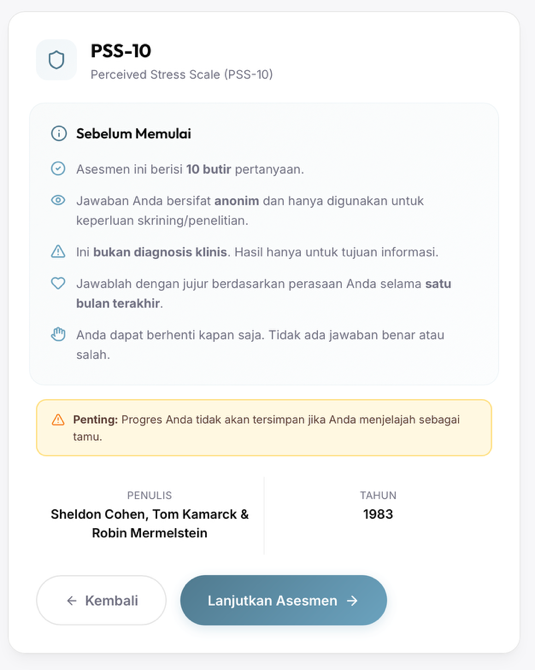
\includegraphics[width=0.9\textwidth]{figures/bukti_13_penyimpanan_sementara.png}
\caption{Bukti Butir 13: Penyimpanan data sementara}
\label{fig:bukti-13}
\end{figure}

\begin{figure}[H]
\centering
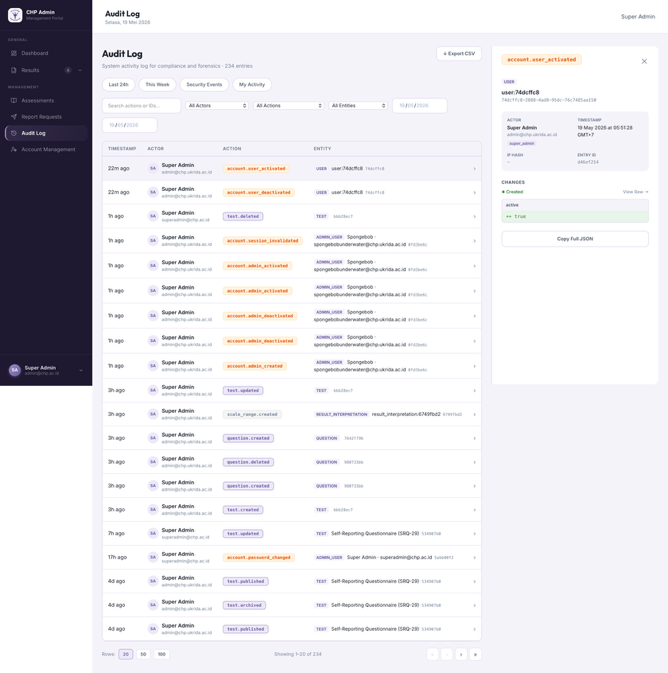
\includegraphics[width=0.9\textwidth]{figures/bukti_14_log_aktivitas.png}
\caption{Bukti Butir 14: Modul log aktivitas}
\label{fig:bukti-14}
\end{figure}

\begin{figure}[H]
\centering
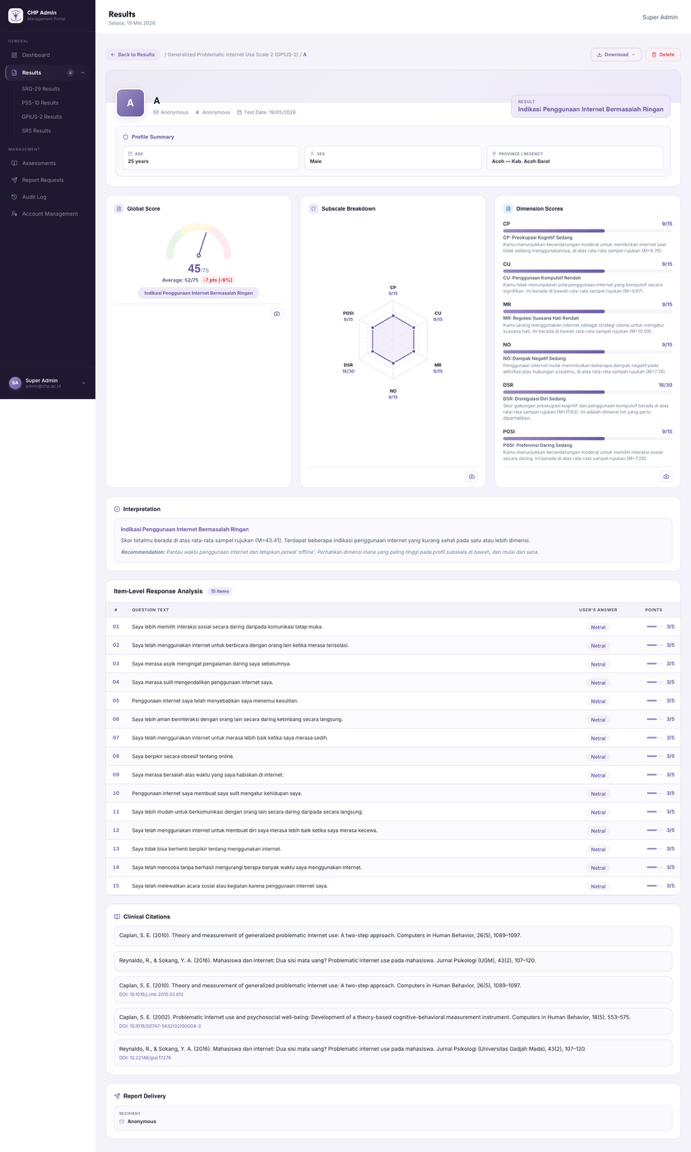
\includegraphics[width=0.9\textwidth]{figures/bukti_15_pelaporan_komprehensif.png}
\caption{Bukti Butir 15: Pelaporan komprehensif}
\label{fig:bukti-15}
\end{figure}

\begin{figure}[H]
\centering
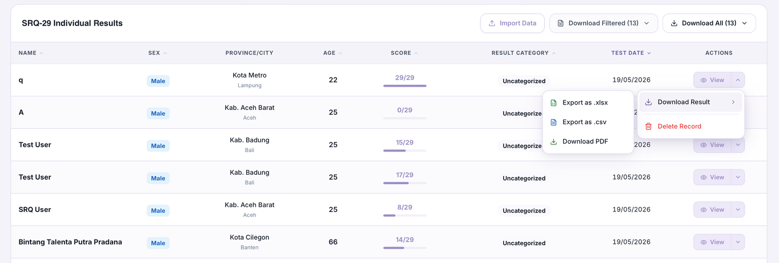
\includegraphics[width=0.9\textwidth]{figures/bukti_16_ekspor_individual.png}
\caption{Bukti Butir 16: Ekspor individual PDF/XLSX/CSV}
\label{fig:bukti-16}
\end{figure}

\noindent\textit{Catatan:} Butir 17 (RBAC bertingkat) tidak disertai tangkapan layar tersendiri karena merupakan logika kontrol akses sisi peladen; pemenuhannya diuraikan pada keterangan Lampiran A dan diverifikasi melalui kasus uji.

\begin{figure}[H]
\centering
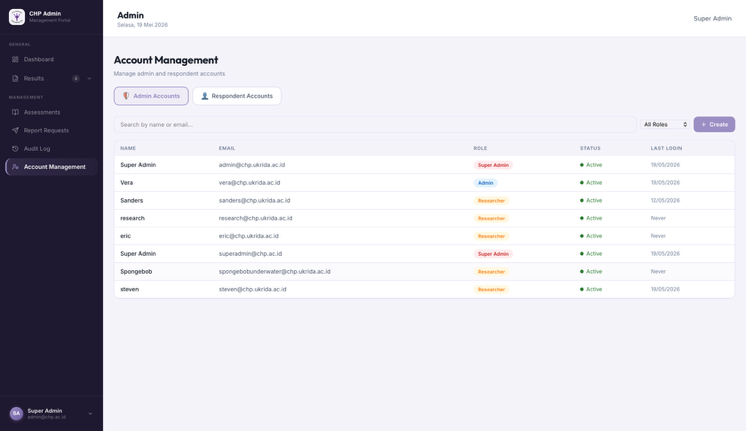
\includegraphics[width=0.9\textwidth]{figures/bukti_18_manajemen_akun.png}
\caption{Bukti Butir 18: Modul Manajemen Akun}
\label{fig:bukti-18}
\end{figure}
